

\chapter{Implementation}
\label{Implementation}
To verify our algorithm we have created a simple, global optimization framework
which enabled us to execute and test all of the algorithms described throughout
this article.

We decided to use Java \cite{java} as a programming language and runtime
environment for this project. 

Using the framework we can find optima of real, mulimodal, multidimensional and
continuous functions. We just need to provide the framework with the concrete
fitness function implementation, and by specifying the problem domain.

The framework principle is to separate the interfaces from implementation.
Our API provides interfaces for evolutionary algorithms, fitness assignment
and fitness deterioration, genetic operators like selection and reproduction,
phenotype, clustering algorithms and many more. This makes it compact,
extensible and easy to introduce new implementations.
For the detailed description of the classes and interfaces see subsection
'Implementation in Java'.  

\section{Architecture}

The project consists of six main packages, which communicates with the
others through clearly specified interfaces and together constitute a
complete, lightweight framework for testing and execution of the global 
optimization algorithms especially the evolutionary algorithms.
\begin{itemize}
  \item \textit{Algorithm module} - central module of the framework. Contains
  implementation of the \textit{Sequential Niching} algorithm as described in
  chapter 2. The main class in the module
  \textit{ki.edu.agh.algorithm.SequentialNichingWithOpticsClustering} is
  responsible for creation of the Spring context and execution of the algorithm. 
  \item \textit{Clustering module} - contains interfaces for clustering
  algorithms and implementation of OPTICS.
  \item \textit{Fitness deterioration module} - contains implementation of
  \textit{FitnessDeterioration} interface. Most important are:
  \textit{ki.edu.agh.deterioration.SimpleGaussianFitnessDeterioration} and 
  \textit{ki.edu.agh.deterioration.WeightedGaussianFitnessDeterioration}.
  \item \textit{Evolutionary Algorithms module} - contains all the necessary
  interfaces for EA, selection and reproduction operators, individuals and
  phenotypes. Implementations of SGA and Evolution Strategy. 
  \item \textit{Printing Modul} - used to print populations and fitness
  landscape during the program execution
  \item \textit{Statistics Utils} - based on JAMA \cite{jama}. This package
  contains many useful statistical functions, e.g. CFA algorithm, covariance
  matrix estimation, multidimensional Gaussian function, fitness deterioration
  untilities.
\end{itemize}

\section{Implementation in Java}
The framework was written to be elegant and extensible. The system's 
modules are loosely coupled and each of system's components has little knowledge of the definitions 
of other separate components (see previous section). This allows for
extensibility in further design. To implement the system we used Spring
\cite{spring} as an application framework, Maven \cite{maven} for project
management and build automation, JUnit \cite{junit} and Mockito \cite{mockito}
for testing and Git \cite{git} as revision control system. 
The source code, configuration files and sample results may be found at 
GitHub \cite{github}: https://github.com/wolny/Fitness-Deterioration

\subsection{Technologies}
\begin{itemize}
  \item Spring \cite{spring} - application framework
  \item Maven \cite{maven} - project management and build automation
  \item Mockito \cite{mockito} - testing framework 
  \item JAMA \cite{jama} - linear algebra package
\end{itemize}

\subsection{Diagrams}

Below you may find class diagrams for each of the module implemented in our
framework. It shows a general overview of the structure of a system: used
classes, their attributes, operations and the relationships between the classes.


\begin{figure}
  \centering
  \fbox{
    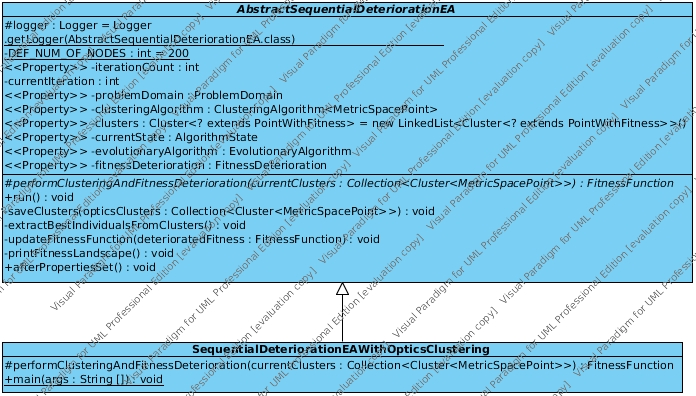
\includegraphics[scale=0.5]{ClassDiagrams/algorithm.jpg}
  }
  \caption{Main algorithm package}
  \label{alg}
\end{figure}

\begin{figure}
  \centering
  \fbox{
    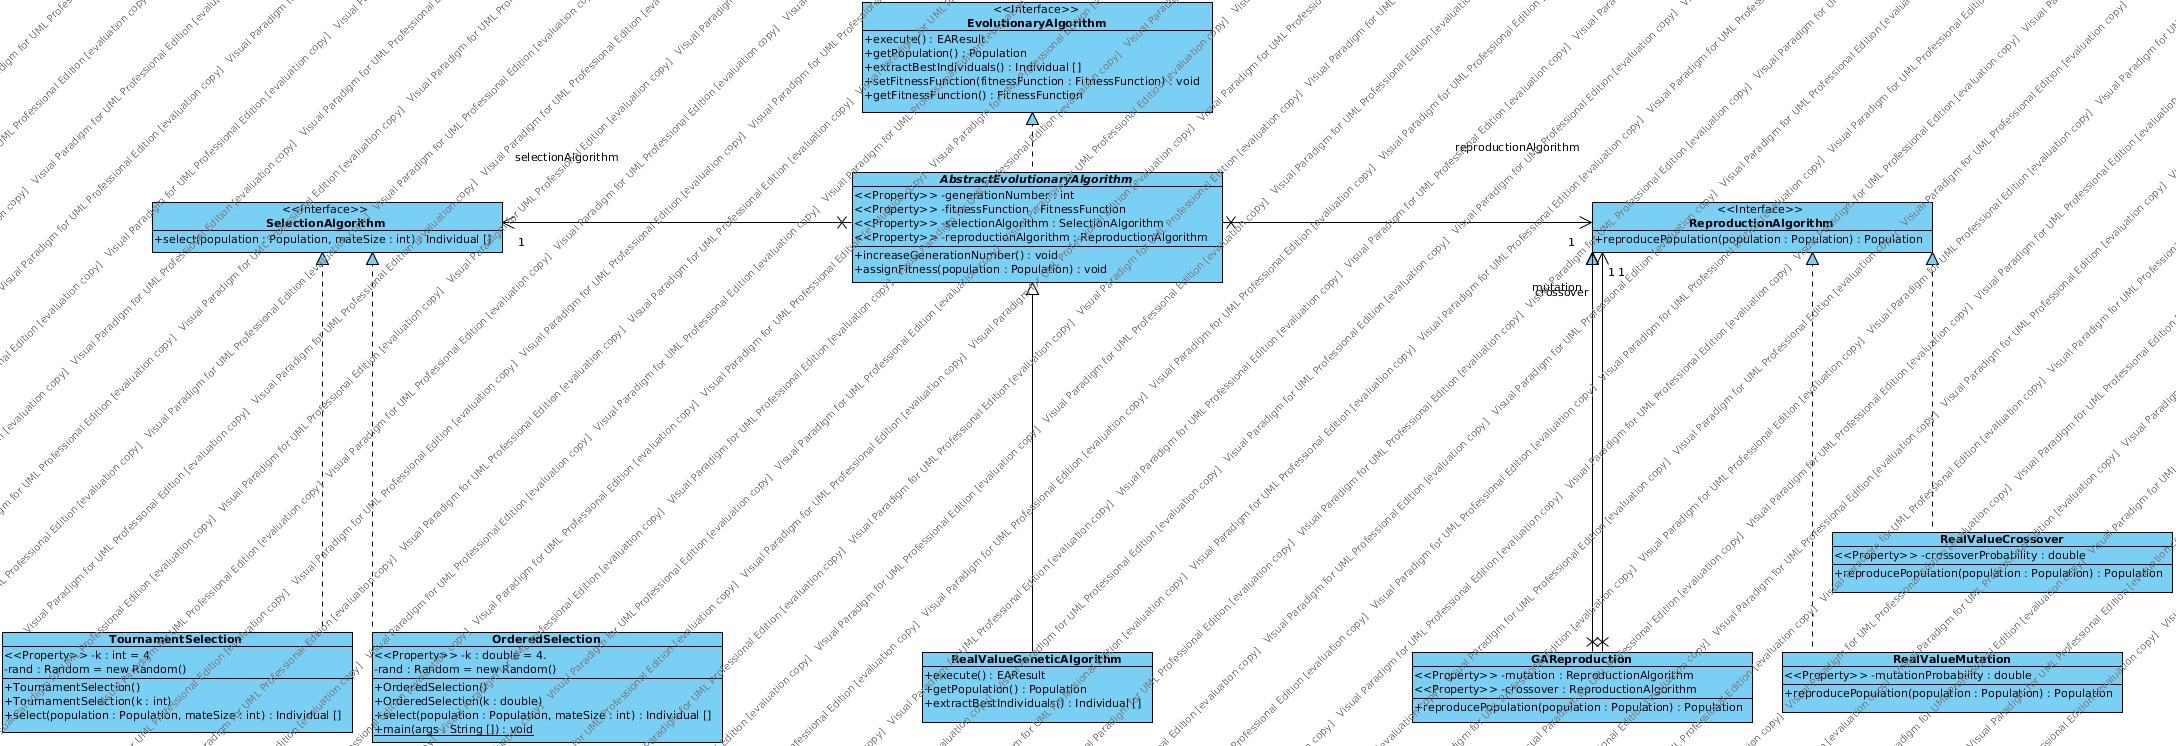
\includegraphics[scale=0.3, angle=90]{ClassDiagrams/EA.jpg}
  }
  \caption{Evolutionary algorithms package}
  \label{ea}
\end{figure}

\begin{figure}
  \centering
  \fbox{
    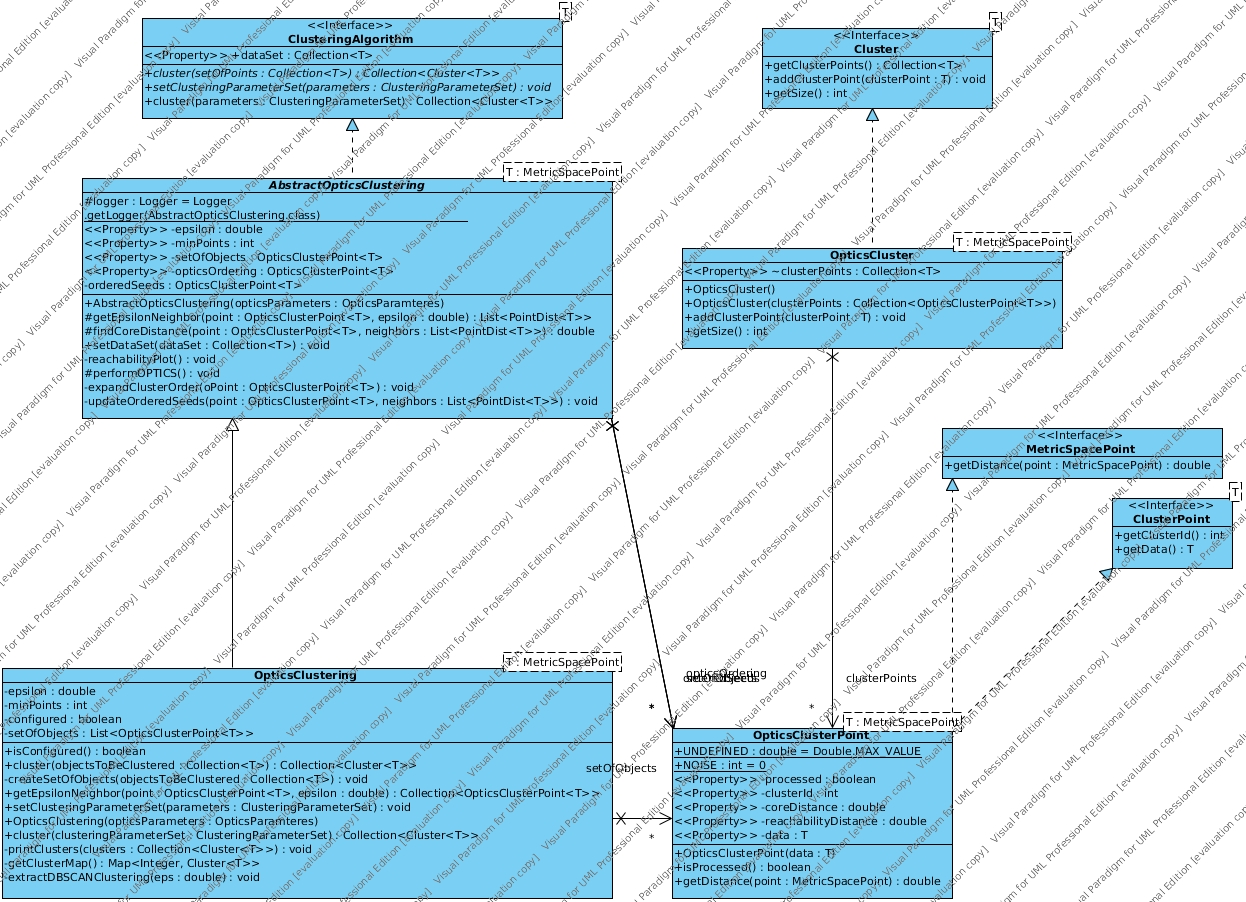
\includegraphics[scale=0.3, angle=90]{ClassDiagrams/clustering.jpg}
  }
  \caption{Clustering package}
  \label{optics}
\end{figure}

\begin{figure}
  \centering
  \fbox{
    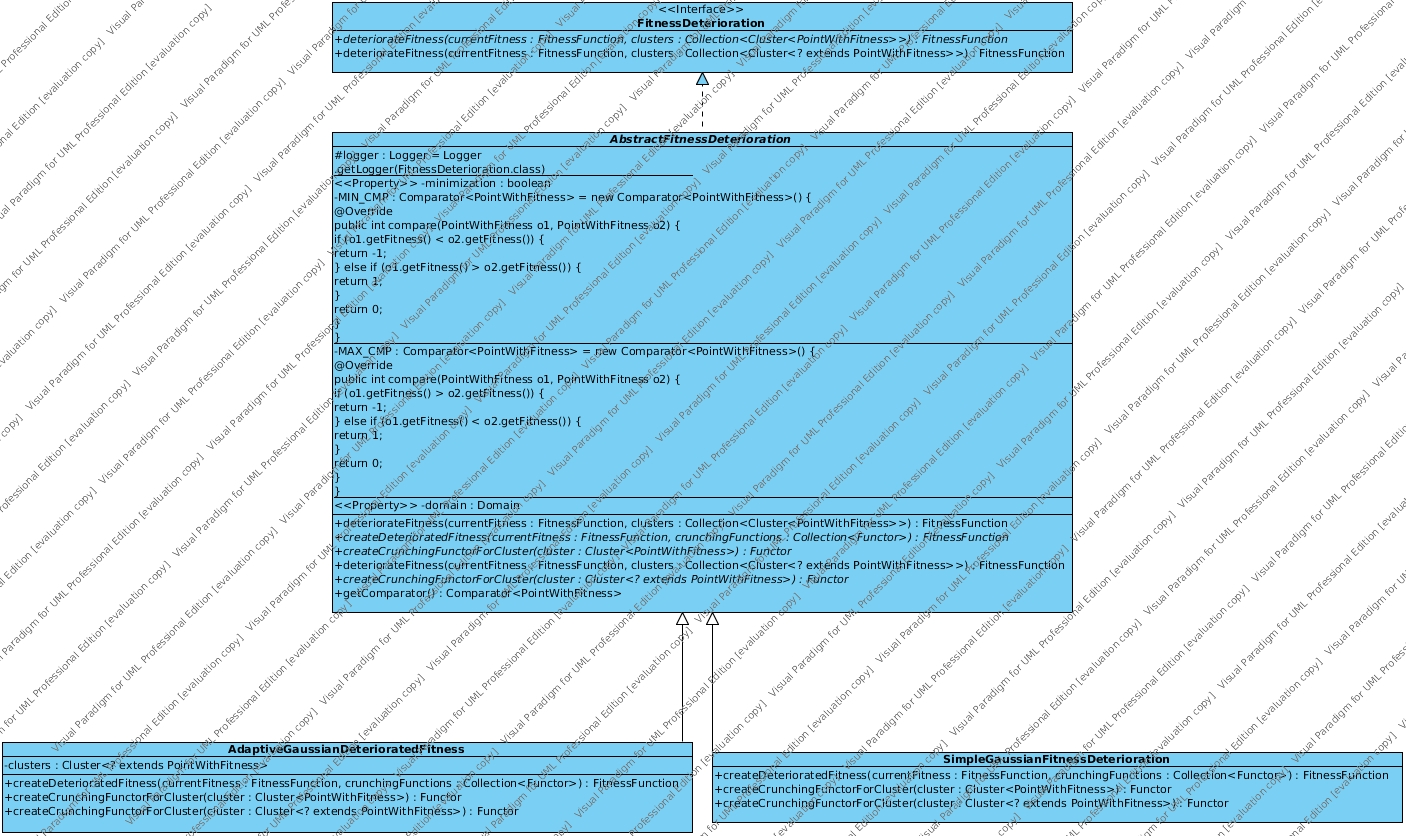
\includegraphics[scale=0.3, angle=90]{ClassDiagrams/deterioration.jpg}
  }
  \caption{Fitness deterioration package}
  \label{fitdet}
\end{figure}

\begin{figure}
  \centering
  \fbox{
    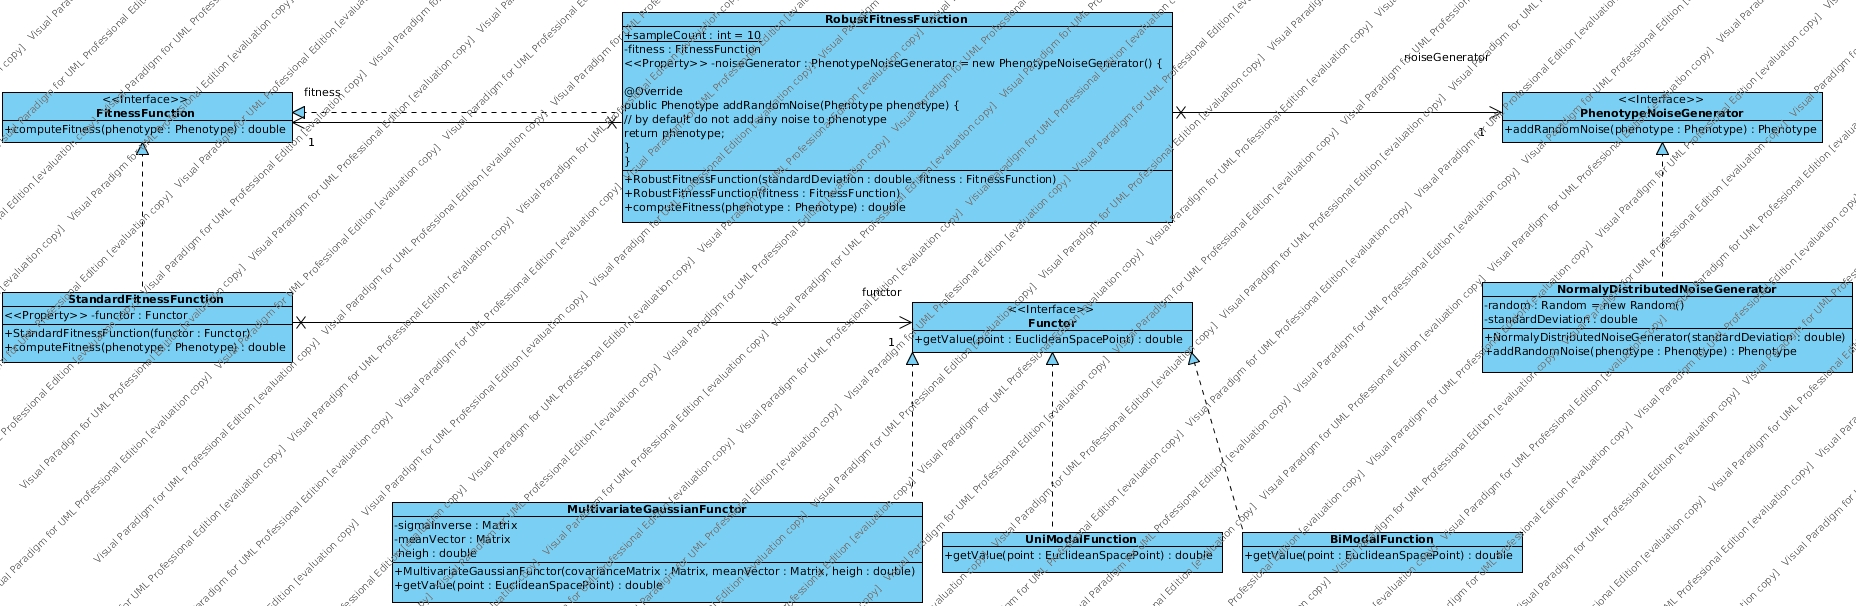
\includegraphics[scale=0.3, angle=90]{ClassDiagrams/fitness.jpg}
  }
  \caption{Fitness and functors package}
  \label{ea}
\end{figure}

\begin{figure}
  \centering
  \fbox{
    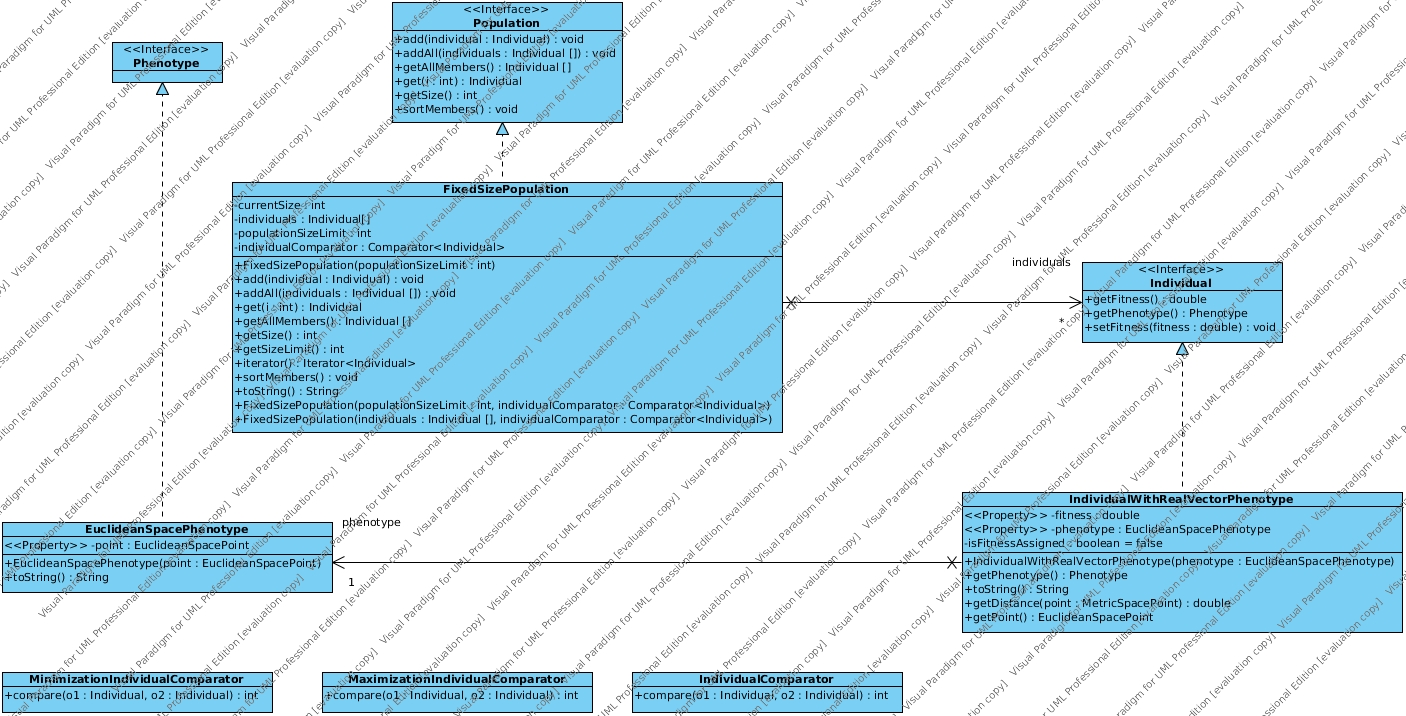
\includegraphics[scale=0.3, angle=90]{ClassDiagrams/population.jpg}
  }
  \caption{Population package}
  \label{ea}
\end{figure}